\documentclass[letterpaper,12pt,oneside]{book}

\usepackage{graphicx}
\usepackage{geometry}
\usepackage{changepage}
\usepackage{tikz}
\usepackage[titletoc]{appendix}
\usepackage{titlesec}
\usepackage{setspace}
\usetikzlibrary{matrix,shapes,arrows,positioning,chains}

\renewcommand{\baselinestretch}{2}
\geometry{left=1.5in,right=1in,top=1in,bottom=1in}

\titleformat{\chapter}[hang]
{\normalfont\Large\bfseries}
{\MakeUppercase{\chaptertitlename}\ \thechapter:}
{0.5cm} {\MakeUppercase}

\begin{document}
	
	%\pagenumbering{roman}
	\frontmatter
	\begin{titlepage}
		\begin{center}
		\textsc{\Large AUTOMATIC GUIDED VEHICLE APPLICATION:}\\[1cm]
		\textsc{\Large PRECISION AGRICULTURE}\\[5cm] 
		\textsc{\Large Xiangnan Gong}\\[5cm] 
		{\large Submitted to the faculty of the School of Informatics in partial fulfillment of the requirements for the degree of Master of Science in Electrical and Computer Engineering, Purdue University \\[0.5cm]Indianapolis, Indiana}\\[0.5cm] 
		{\large \today}
		\end{center}
		\newpage
		\begin{center}
			THE PURDUE UNIVERSITY GRADUATE SCHOOL \\
			STATEMENT OF CHOOSE THESIS TYPE APPROVAL
			\\[2cm]
		\end{center}
		
		
		Dr. Lingxi Li, Chair
		
		\hspace{1cm} Department of Electrical and Computer Engineering
		
		Dr. Brain King 
		
		\hspace{1cm} Department of Electrical and Computer Engineering		
		
		Dr. Maher Rizkalla 
		
		\hspace{1cm} Department of Electrical and Computer Engineering	\\[2cm]
		
		
		Approved by:
		
			
		
	\end{titlepage}
	
	\begin{spacing}{1.5}
		\setcounter{tocdepth}{3}
		\renewcommand\contentsname{TABLE OF CONTENTS}
		\tableofcontents
		
		\renewcommand\listfigurename{LIST OF FIGURES}
		\listoffigures
		\addcontentsline{toc}{chapter}{LIST OF FIGURES}
		
		
		\renewcommand\listtablename{LIST OF TABLES}
		\listoftables
		\addcontentsline{toc}{chapter}{LIST OF TABLES}
	\end{spacing}
		
		
		
	\chapter*{Abstract}
	\addcontentsline{toc}{chapter}{Abstract}
		Nowadays, there are many types of Automatic Guided Vehicle (AGV) running in different field of industries. Typically their job is moving raw materials or parts around the manufacturing facility. And they can be very accurate in working by following the guide from the wires in the floor, magnets, laser, or vision. However, they all require the an indoor condition. Therefore, the purpose of this thesis report is to discuss the implement of the outdoor-AGV. An outdoor-AGV has much more constraints than indoor ones. The environment indoor can be easily controlled while the outdoor cannot. The problem could be rough ground, no pre-set guiding wire or magnets, vision blocking by dust, and so on. The solution, which will introduce in this paper, to achieve the outdoor AGV is guiding by laser. In addition, a buffer will be installed to stabilize the cargo or others working devices, to prevent them from the shaking due to the rough ground. To be more specific, a prototype will be built to simulate the working of seeder. In agriculture, it is very important to plant corns in a straight line. It benefits not only in absorbing sunlight and ventilation, but also reduce the work of irrigation, fertilizing, and harvest. Since a straight line of corn also mean a straight line of aisle. Furthermore, to achieve unmanned agriculture, a corn field with straight line of aisle will be a good condition for other agriculture robots. 
	 

	\mainmatter
	\setcounter{secnumdepth}{3}
		\chapter{Introduction}
		\section{Introduction to subject}
		
		Since nineteenth century, machines have been playing a more and more important role in every aspect all around the world. Especially in the modern factories, a few workers are capable to accomplish the job that used to require hundreds of skillful workers to do with a well-designed mechanical production line. 
		Specifically, what machines brought to us is not just the efficiency, but also the accuracy and the reliability. Therefore, automatizing the production, which in another word, replace human workers with robots is imperative for every production plant. 
		
		In 1950s, the first Automatic Guided Vehicle (AGV) was introduced by Barrett Electronics to handle materials for a production line. \cite{olmi2011traffic} It was a just a tow truck following a wire in the floor at that time. However, after decades of development, AGVs are able to help to achieve the unmanned production line in many factories nowadays. Modern AGVs with build-in microprocessors can be controlled by computer. Therefore they are not only the machine that move heavy materials around, but also significantly accurate and reliable. A typical AGV can have over 1000 pounds load capacity, in addition, the tracking accuracy is just +/- 1.27 $cm$. \cite{KESH} 
		
		There are many types of AGVs, such as towing vehicle, unit load carrier, forklift trucks and so on. They are all running around the factories by following the guidance system. Generally, the guidance could be pre-rooted wire, magnate, or colorless florescent particles painting. All of these AGVs are pretty accurate, but they can only work indoor. Wires and magnates need to be planted underground, or paintings need to be paint on the concrete tiled floor for guidance. The environment of indoor can be well controlled, while outdoor cannot. The outdoor environment is very complicated and unpredictable. The ground could be rugged, wet, or sleepy. The weather could be exposure, cold, or rain. And the interference could be dust, lightness, or the Earth magnetic field. This paper will provide a solution to bring AGVs from indoor to outdoor, and introduce AGV to the field of precision agriculture.
		
		\section{Importance of subject}
		
		Labor is one of the most significant factors of agriculture. With the help of farm machinery, the total amount of labor dedicated for farming has decreased by about 30 percent for hired labor and about 40 percent for self-employed labor from 1982 to 2007. Moreover, the farm output increased by 35 percent (Table 1.1) while the total amount of labor dedicated to farming was decreasing. \cite{o2011changing} %So the machines are really good helpers to farm. 
		\begin{table}[ht!]
			\begin{center}
				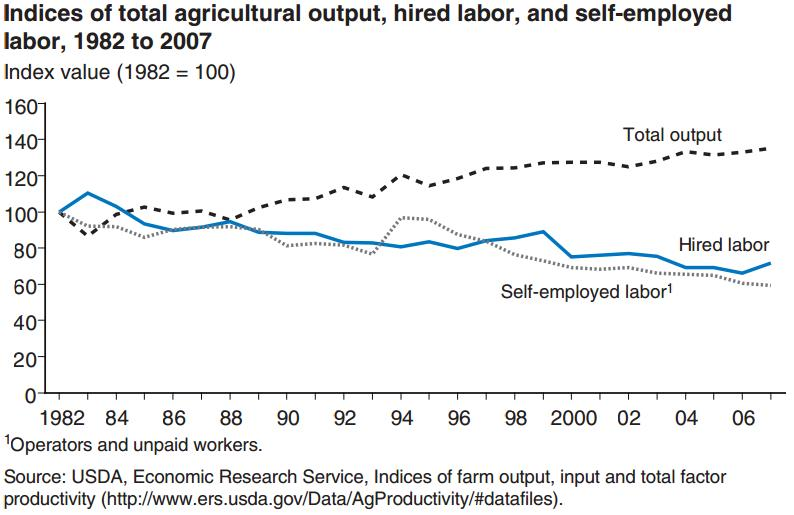
\includegraphics[scale = 0.7]{laborandoutput.jpg}
				\caption{The change labor and output in agriculture}
			\end{center}
		\end{table}
		Undoubtedly, the usage of farm machinery not only lower the amount of labor, but also increase the productivity. 
		
		In late of 20th century, Pierre Robert proposed, developed, and popularized precision agriculture. \cite{mcbratney2005future} Most of the farm machinery now has the GPS, which stands for Global Positioning System, on board because of his contribution. It is very easy to plant all corps in nicely columns with the GPS guidance system. The GPS mounted farm machinery did a great job in the past few years, but there is an error. The accuracy of the original GPS is typically about a few meters. Fortunately, there was a technology that have improved the accuracy to $\pm$ 10 $cm$ which already widely in use. \cite{thuilot2002automatic} Although this $\pm$ 10 $cm$ accuracy is acceptable with most popular 76.2 $cm$ row spacing, not for 50.8 $cm$ or 38.1 $cm$ row spacings that will be used in the future. \cite{fawcett2014farm} In fact, there is a place has a even higher requirement,which is the experiment field. The objective of the experiment field is to find the high quality breed of crops. Therefore, it is extremely important to keep the growth environment of every plant at the same level. The position to seed the experiment field is strict. Every plant should keep the same distance to each other, which is the precondition to provide every plant the same amount of water, sunlight, fertilizer, and carbon dioxide. Failure to do this will cause the result of the experiment is meaningless. Without any shadow of doubt, it is very necessary to have an outdoor AGV working with as high accuracy as the indoor ones.
		
		
		\section{Knowledge gap}
		For thousands of years, farming is one of the most important method to harvest food. It is a big leap from the traditional farming, that farmer could only get help from cattle or horses, to the modern farming, that farmer could get help from farm machinery. It is possible to satisfy the food demand of explosive growth of world human population because of the developing of farming technology. From the current situation in the United States, the products of modern farming is not only able to full fill the food demand of the United States, but also have a huge surplus. For example, more than 70 percent of the volume of U.S. production of Cotton and Tree nuts were exported from 2011 to 2013 (Table 1.2). And the overall average annual export share of U.S. agricultural production is 20 percent since 2000. \cite{Exports}
		\begin{table}[ht!]
			\begin{center}
				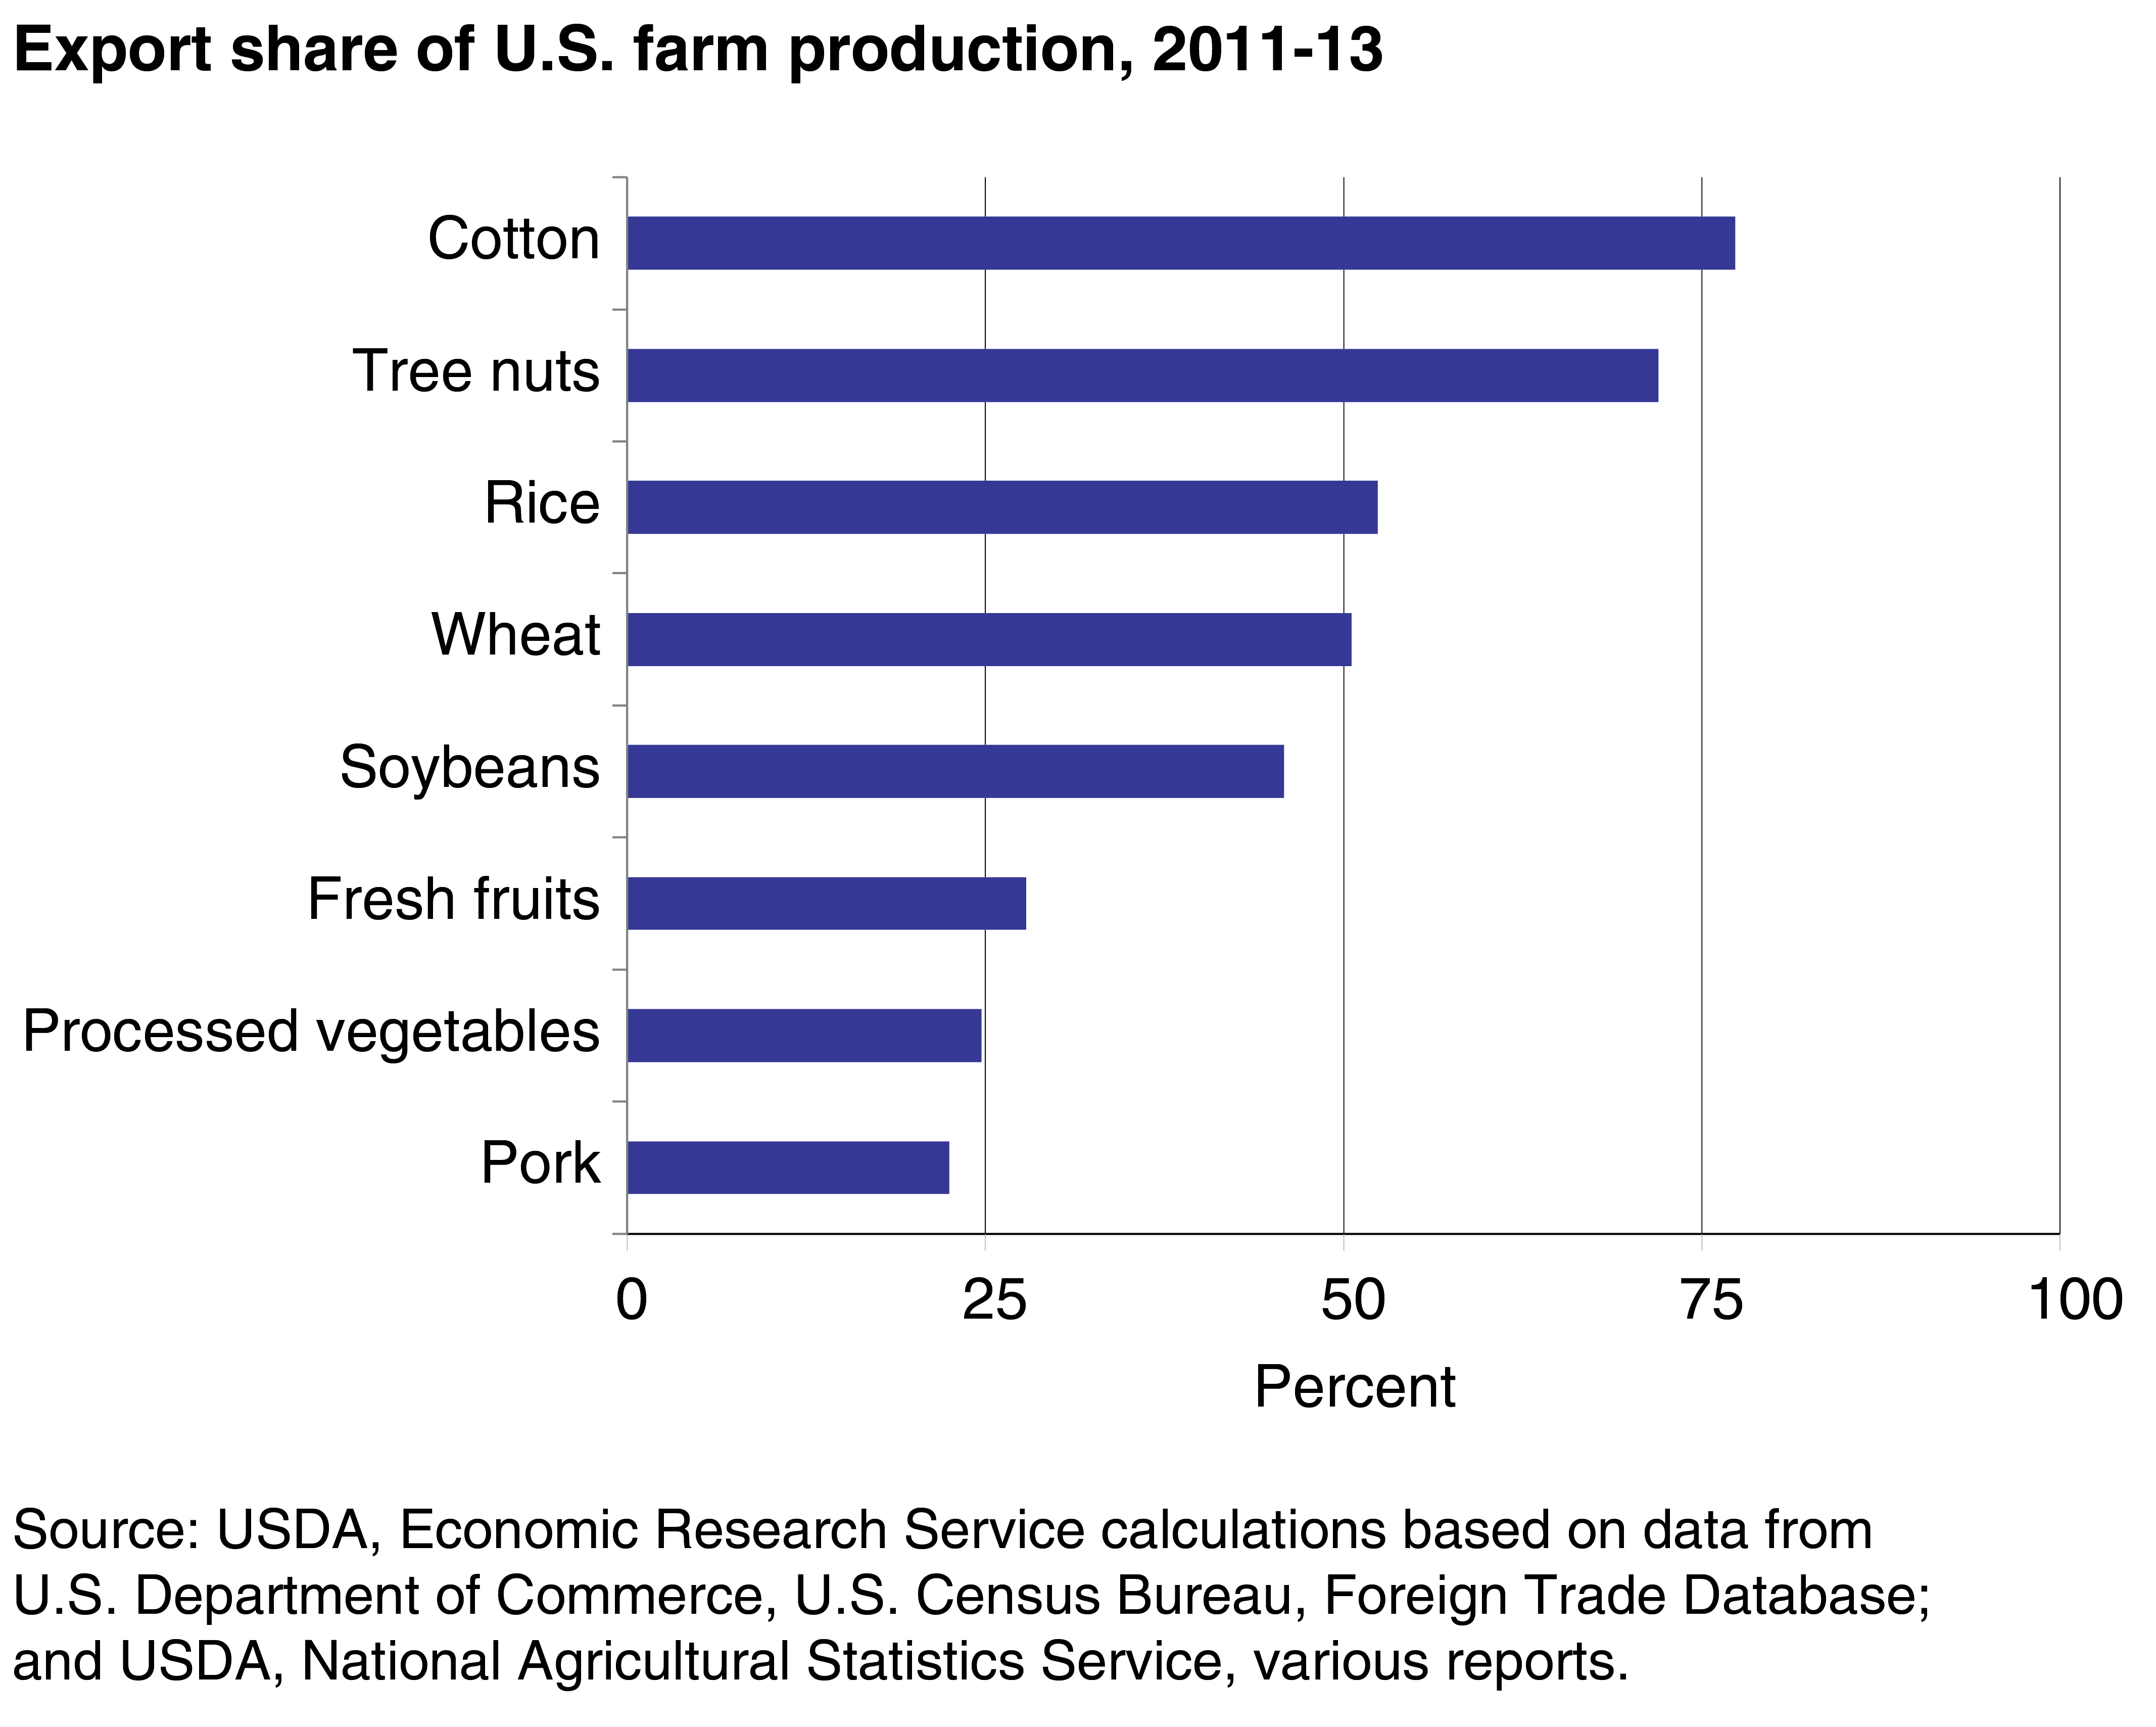
\includegraphics[scale = 0.4]{cropexport.png}
				\caption{Export share of U.S. farm production, 2011-13}
			\end{center}
		\end{table}
		Since there is no food shortages in the U.S., the technology of farm machinery seems to be more than enough. However, there are many other places in the world that is very hard to grow crops, because the farming conditions are totally different compare to the north America. For example, the water scarcity in West Asia and North Africa is a well-known problem. The world average annual per capita renewable supplies of water was about $7000 m^{3}$ in 1999, however, it was below $1500 m^{3}$ in West Asia and North Africa countries at the same time. More seriously, this level was $3500 m^{3}$ in 1960 and it was expected to continuously decrease to less $700 m^{3}$ by the year of 2025. \cite{margat1999water} One of a good solution for the water scarcity is to use the micro-irrigation, to be more specifically, drip irrigation (Figure 1.1). 
		\begin{figure}[ht!]
			\begin{center}
				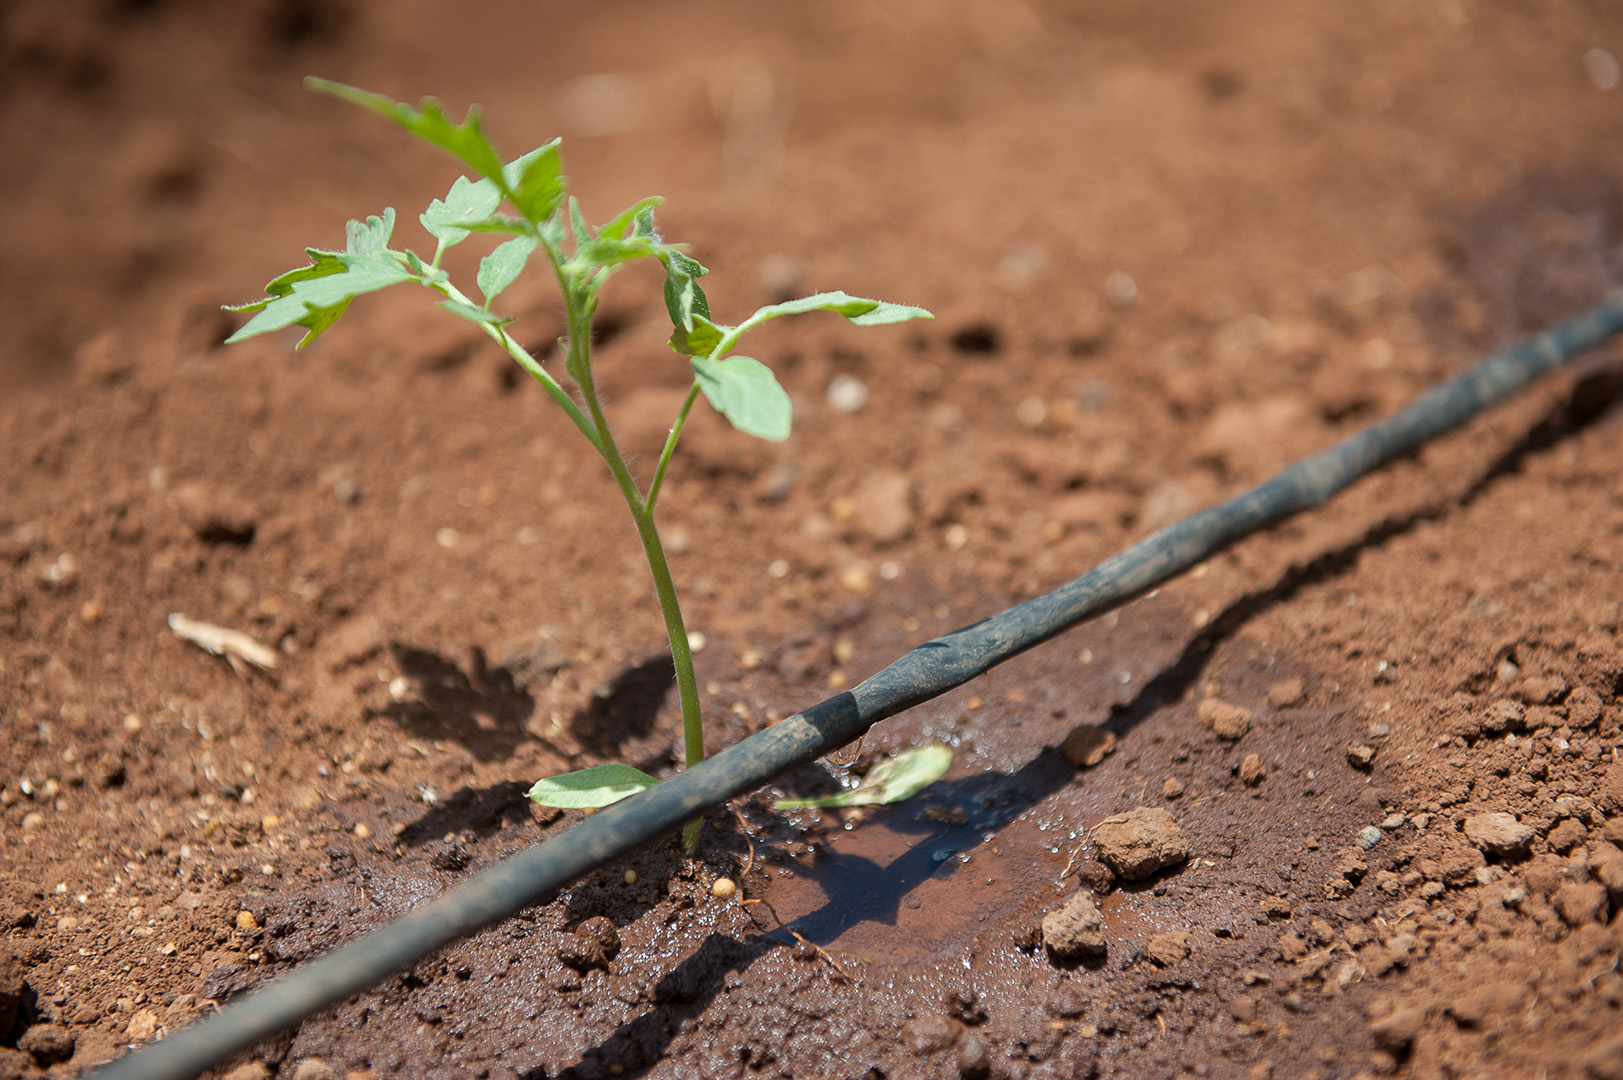
\includegraphics[scale = 0.25]{drip.jpg}
				\caption{Drip Irrigation}
			\end{center}
		\end{figure}
		Some advantages of micro-irrigation include improved water and nutrient management, potential for improved yields and crop quality, greater control on applied water resulting in less water and nutrient loss through deep percolation, and reduced total water requirements. \cite{phene1986advantages} Unfortunately, the applications of micro-irrigation is also limited. Mostly, micro-irrigation was used on permanent plantings such as trees and vines. The reason that not using them on the field crops is that it needs to be installed and removed at the beginning and the end of each growing season. Furthermore, field corps are different from trees and vines, their height is low, so the working zone is close to the ground. Therefore, the drip tubes make the other fields operations to become difficult than it used to be. A improved method to make it possible to use the micro-irrigation on the field corps is to bury the tubes underground. \cite{camp1998subsurface} Although the tubes neither affect the field operations nor need to be reinstalled every growing season, the position of drip spot is fixed once it was buried. So the problem turns into planting crops in the right position, which can be solved by the outdoor AGV that this paper introduced. 
		
		\chapter{Background}
		
		\section{Current AGVs}
		The most popular guidance systems applied on current indoor AGVs are wire-guided, Optical, inertial, infrared, laser, and teaching type. \cite{KESH}
		\begin{itemize}
			\item Wire-Guided:
			\begin{itemize}
				\item An energized wire is rooted along the guide path. 
				\item The antenna of the AGV follows the rooted wire.
			\end{itemize}
			The outdoor crop field is very large compared to the indoor factories. It is too expensive to root wire under ground in advance. And because of the variety of the temperature and humidity, the wire is easy to be eroded.
			\item Optical:
			\begin{itemize}
				\item Colorless florescent particles are painted on the concrete/tiled floor. 
				\item Photosensors are used to track these particles.
			\end{itemize}
			It is impossible to paint the colorless florescent particles on the soil.
			\item Inertial:
			\begin{itemize}
				\item The guide path is programmed on a microprocessor which is fixed on the AGV. 
				\item Sonar system is incorporated for finding obstacles.
			\end{itemize}
			Sonar system cannot be used as a guidance system in an open area.
			\item Infrared:
			\begin{itemize}
				\item Infrared light transmitters are used to detect the position of the vehicle.
				\item Reflectors are affixed on the top of vehicle to reflect the light.
			\end{itemize}
			It is hard to detect the position of the vehicle by using infrared light transmitters in under sunlight.
			\item Laser:
			\begin{itemize}
				\item Laser beam is used to scan wall-mounted bar-coded reflectors.
				\item Accurate positioning can be obtained.
			\end{itemize}
			This is using for a very close distance to enhance accuracy.
			\item Teaching type:
			\begin{itemize}
				\item AGV learns the guide path by moving the required route.
				\item Sends the information to the host computer.
			\end{itemize}
			The outdoor ground is rough and unpredictable. It is hard to stay in the planned route by just memorizing it. Because small errors of moving on rough ground cumulates to big errors. 
		\end{itemize}
		It is obvious that none of the indoor AGVs guidance systems are suitable for outdoor AGVs.
		
		\section{Related researches}
		\subsection{Sound guidance}
		The sound guided vehicle was implemented with one buzzer ,which mounted on the vehicle ,and three sound receivers. Just like human can detect the position of sound source by using two ears, there was a algorithm designed with the same principle to detect the position of the buzzer. (Figure 2.1) 
		\begin{figure}[ht!]
			\begin{center}
				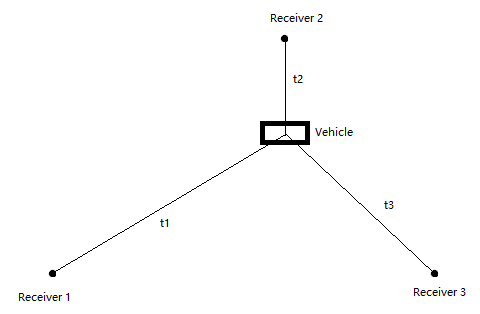
\includegraphics[scale = 1]{soundguided.png}
				\caption{Sound Guidance System}
			\end{center}
		\end{figure}
		
		On the vehicle side, the buzzer keeps emanating a cyclical audio pulse with specific signal frequency. On the guidance system side, computer recognizes and picks up the audio pulse from all three receivers. According to the time differences of receiving the same pulse, the developed algorithm is able to locate position of the vehicle. With knowledge of the vehicle location, guidance system can send the action command. The result of the experiment shows that the error is about 1 - 5 $cm$ under a velocity of 6 - 12 $cm/s$.\cite{yuping2011sound}
		
		Most of agricultural operation is under an open area condition. Typically the a single crop field is beyond 200 $m$ in length or width. It is difficult to recognize a sound signal with this range of distance.  High resolution microphone must be used so that it can pick up weak signal from a farther distance. However, solving the long distance problem is not only just using a more expensive microphone to pick sound. The average speed of sound is 340 $m/s$ in air, and the actual speed vary along the density of air. In another word, altitude, atmospheric pressure, and humidity all can change the speed of sound. And because of the microphone is more sensitive, noise filtering is also another challenge. Hence, sound guidance is not suitable for agriculture applications.
		
		\subsection{Vision guidance}
		Vision guidance is based on the information gathered by camera and dead reckoning. The developed algorithm first find a specific point in the frame, and then stare on it. From the movement of this point, the movement of vehicle is able to be reckoned. The result of the experiment shows that the error is about $5 cm$ under a velocity of $8 m/s$. \cite{jiang2006algorithm} However, the vehicle was tested on asphalt road with painted lines. The ground of farm land is rough and slippery, and there is not painted line. Therefore, vision guidance is a good choice for cars but not for agriculture applications.
		
		\subsection{GPS}
		GPS guidance system is one of the most reliable guidance system. There are many advantages such as low cost, portable, and able to work at any places without any pre-installation. However, the accuracy of GPS is always a problem for agriculture. An experiment in 2014 had a result that 
		\begin{adjustwidth}{0.5 in}{}
			\textit{almost half (49.6\%) of all ≈68,000 GPS points recorded with the Qstarz Q1000XT GPS units fell within 2.5 m of the expected location, 78.7\% fell within 10 $m$ and the median error was 2.9 $m$. The four different types of areas showed considerable variation in the median error: 0.7 $m$ in open areas, 2.6 $m$ in half-open areas and 5.2 $m$ in urban canyons.} \cite{schipperijn2014dynamic}
		\end{adjustwidth}
		According to this research, the median error for GPS is 0.7 $m$ in open areas which is 70 $cm$. This accuracy is obviously not enough for field operations because the row spacing is 76.2 $cm$.
		
		\subsection{Improved GPS guidance}
		An improved technology for GPS, CP-DGPS (Carrier Phase Differential GPS) also named RTK GPS (Real-Time Kinematic GPS), brought the accuracy to centimeter lever. This RTK GPS have two receivers. One of them it call \textit{reference}, another one is call \textit{rover}. \textit{Reference} is a receiver that installed to a fixed position. It always stay at the same position and permanently receives the satellite signals, calculates its ‘GPS’ position and determines the difference with the coordinates attributed to its own position. The \textit{rover} is mobile and placed to where it is needed to be. It receives both GPS signal from satellites and the correction values from \textit{reference} via radio signal. \cite{lambiel2004contribution} And base on the experiment had on a farm tractor, the error is lower to 10 $cm$. \cite{thuilot2002automatic} This error is acceptable with most popular 76.2 $cm$ row spacing now, but not for the 50.8 $cm$ or 38.1 $cm$ row spacing in the future. \cite{fawcett2014farm} 
		
		\subsection{Sliding correction}
		The ground condition of corp field is unpredictable. So the 10 $cm$ accuracy for GPS does not equivalent to 10 $cm$ accuracy for trajectory. Unlike the asphalt road, soil cannot provide constant fraction on every tires of vehicle. Sliding is a significant problem that causes trajectory error. Therefore an algorithm for sliding estimation was developed. Two inclinometers were installed on the vehicle to collect data. (Figure 2.2) 
		\begin{figure}[ht!]
			\begin{center}
				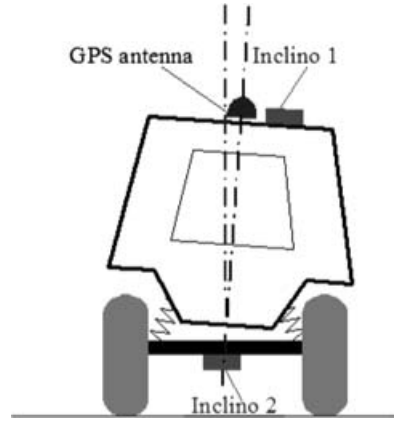
\includegraphics[scale = 0.5]{slidingcorrection.png}
				\caption{Position of inclinometers}
			\end{center}
		\end{figure}
		From these two tilt angles, the design algorithm can estimate the sliding and then give feedback to control system as correction. The result from this research shows that the actual trajectory error is within $\pm$ 15 $cm$. \cite{lenain2006high}
		
		\section{Research question}
		Based on the related researches,achieving precision agriculture is not only to improve the accuracy of the position of farm machinery, but also to improve the accuracy of trajectory. With the localization technology, correction could be made once the vehicle off the track; with the sliding estimation technology, correction could be made once the tire slid. All the researches have done were trying to find the exact position of the vehicle or to estimate sliding then make the correction. However, making correction means errors already occurred. To prevent error from happening, an additional device and guidance system was designed.  
		
		\section{Intended project}
		
		Driving on the farm field faces unpredictable ground conditions all the time, such as rocks, mounds, slide, rabbit or rat holes. It is impossible for tractors to drive through every thing without deviating the planned track. However, it is possible to have the attachments of the tractors always stay on the planned track. The design is to install a buffer on the tractor attachments. (Figure 2.3)
		\begin{figure}[ht!]
			\begin{center}
				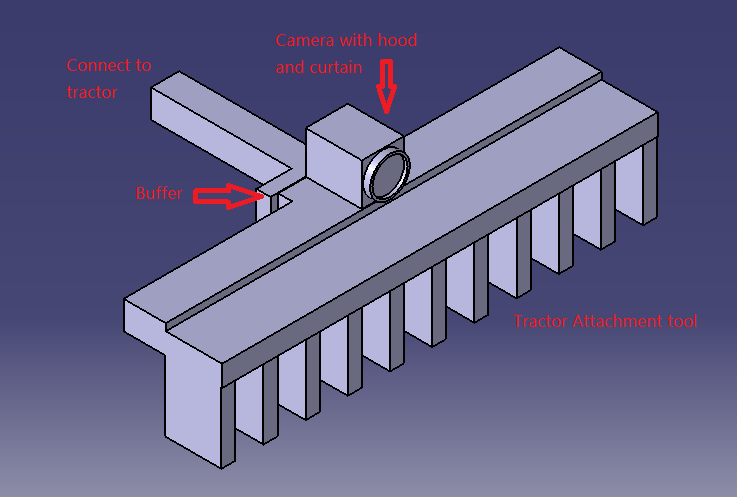
\includegraphics[scale = 0.8]{attachmentwithbuffer.png}
				\caption{Tractor with buffer installed}
			\end{center}
		\end{figure} 
		The buffer allows the tractor to have some left or right displacement by providing an offset in the opposite direction to the attachment. Therefore, as long as the tractor moves in a right direction and have an accuracy that within the offset range of the buffer. The attachment is able to work in a relatively stationary condition. 
		
		According to the related researches, vision guidance has been chosen to use as the guidance system for the buffer, because camera is a low cost device, and the imaging process algorithm is easy to be updated in the future implement. In the paper, an additional laser pointer is used as a stable reference. The laser pointer is placed at the end of rows facing to the back of tractor to provide the guidance. (Firuge 2.4) So that the buffer can provide the proper offset by observing the laser beam. It is expected to improve the accuracy dramatically from 10 $cm$ to about 2 $cm$. 
		\begin{figure}[ht!]
			\begin{center}
				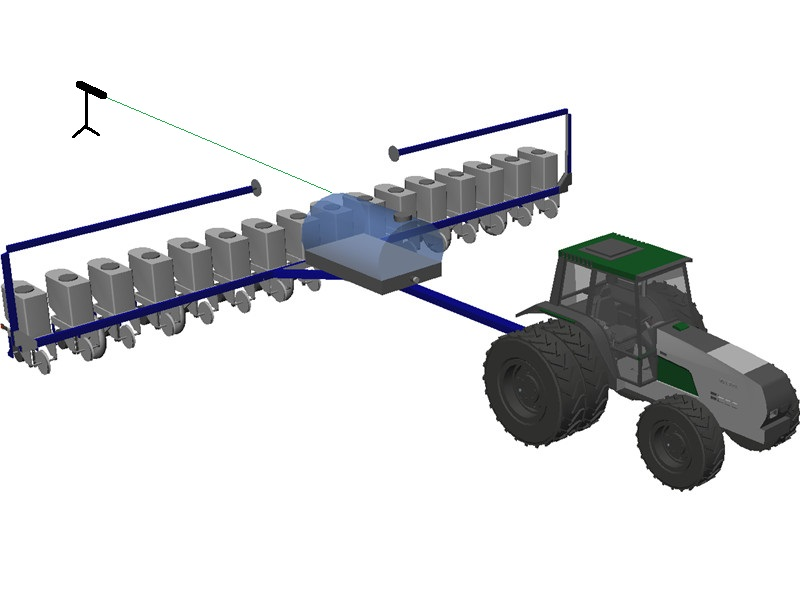
\includegraphics[scale = 0.6]{tractor.jpg}
				\caption{Laser Guidance}
			\end{center}
		\end{figure}
		
		\chapter{Design}
		The buffer is designed to be installed on the tractor attachment. And the frame of all the tools on the attachment should connect to the buffer so that they are able to move along with the buffer. At the beginning, the camera on the buffer sees the laser spot and set up the initial position. As the tractor moving, the buffer will keep maintaining the laser spot in the original position. In another word, once slide occurs on the tractor, buffer will shift the tools on the attachment to the opposite direction to prevent them from shifting. The algorithm is showing on the flow chart. (Figure 3.1)
		% Define block styles
		\tikzstyle{decision} = [diamond, draw, text width=2.5cm, text badly centered]
		\tikzstyle{block} = [rectangle, draw, text width=3cm, text centered, rounded corners, minimum height=1cm]
		\tikzstyle{line} = [draw, -latex']
		\begin{figure}
			\begin{center}
				\begin{tikzpicture}
				\node[block](start) {Start};
				\node[block, below = 1 of start] (origin) {Initialize Position};
				\node[coordinate, below = 1cm of origin] (cycle) {};
				\node[decision, below = 2 of origin] (L) {Is left slide decteted?};
				\node[block, left = 2 of L] (goR) {Provide right offset};
				\node[decision, below = 1 of L] (R) {Is right slide decteted?};
				\node[block, left = 2 of R] (goL) {Provide left offset};
				\node[coordinate, left = 1cm of goR] (left) {};
				\node[coordinate, below = 1cm of R] (bottom) {};
				
				\path [line] (start) -- (origin);
				\path [line] (origin) -- (L);
				\path [line] (L) -- node [anchor = south] {yes} (goR);
				\path [line] (goR) -- (left) |- (cycle);
				\path [line] (L) -- node [anchor = east] {no} (R);
				\path [line] (R) -- node [anchor = south] {yes} (goL);
				\path [line] (goL) -| (left) |- (cycle);
				\path [line] (R) --  node [near start, anchor = east] {no} (bottom) -| (left) |- (cycle);
				\end{tikzpicture}
				\caption{Flow Chart}
			\end{center}
		\end{figure}
		\section{Materials and instruments}
		This buffer is designed to be a implement base on current tractor attachments. In this paper, a prototype was developed for designing and experimental purpose. (Figure 3.2) 
		\begin{figure}[ht!]
			\begin{center}
				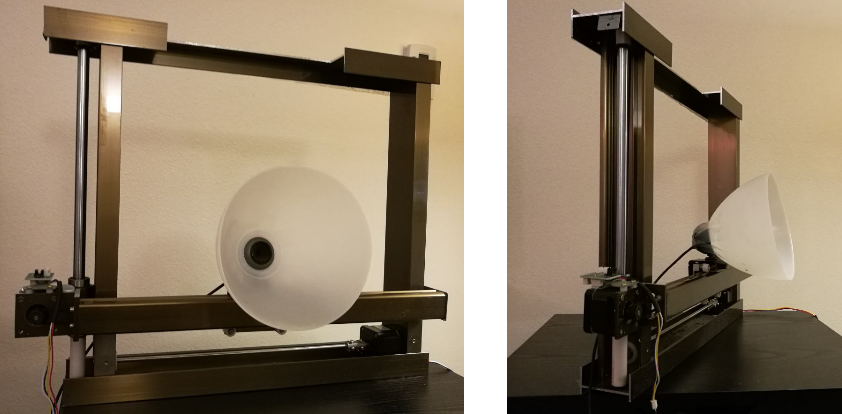
\includegraphics[scale = 0.6]{prototype.png}
				\caption{prototype}
			\end{center}
		\end{figure}
		A camera is installed on the top facing backwards to gather image information. A laser Pointer is placed at the end of row, facing the direction that same with the tractor moving and aiming the camera. Stepper motors are installed on the frame to provide offset for the tractor attachments. And a Raspberry Pi is used as central processor to analysis the information gathered by camera and give the action commands to stepper motors. In addition, stepper motor drivers boards are installed to transform the digital control signal to stepper motors input. The power supply was designed to use the battery of the tractor. So there is no battery in this prototype. All the parts are listed in Table 3.1.
		
		\begin{table}[ht!]
			\begin{center}	
				\begin{tabular}{|l|p{1.5cm}|p{4cm}|l|l|l|}
					\hline
					Part Name & Vendor & Description  & Unit Cost & Qty. & Total Cost \\ \hline
					Camera & Logitech & 480P WEBCAM & - & - & -\\ 
					\hline
					Stepper Motor & ECOSS INC & Came with frame & - & - &\\ 
					\hline
					Driver boards & DROK & L298N Motor Drive Controller Board & 6.99 & 1 & 6.99\\
					\hline
					Microprocessor & CanaKit & Raspberry Pi 2 with Starter Kit & 84.99 & 1 & 84.99\\
					\hline
					Frames & ECOSS INC & X-Y Stage Table Bed &  169.00 & 1 & 169.00\\
					\hline
					Wires & Phantom YoYo & 40p Male to Female 40p Female to Female & 4.40 & 1 & 4.40\\
					\hline
					Camera Hood & - & Lampshade & - & - & -\\
					\hline
					Curtain & - & Foam Board & - & - & -\\
					\hline
					Laser Pointer & Fowll & 532 nm Green Laser & 22.99 & 1 & 22.99\\
					\hline
					Power Supply & Goodwill & Used Charger & 1.99 & 2 & 2.98\\
					\hline
				\end{tabular}
				\caption{Parts List}
			\end{center}
		\end{table}
		
		%对现有农机进行改装,所以成本低。现在实验阶段使用的是,电源,树莓派,摄像头,步进马达,框架,幕布,激光。(做图表,列出成本)
		
		\section{Laser guided}
		
		Laser pointer is a economic and efficient way to provide a straight and stable reference. Thus, laser guidance is selected to be the guidance system. In order to observe a clear laser reference in a far distance, high power laser is the best choice. On the other hand, there is the safety problem to the laser pointer. High power laser pointers could damage retina if the distance is too close. Base on this safety problem, the restriction of power of laser pointer should be the lower the better. To achieve both low power and far range, the color of laser was chosen to be green. Since green light has shorter wave length than the red light, it is able to spread farther than red light with the same power. According to the from Table 3.2, the maximum eye hazard distance of a 5 $mW$ green laser pointer is only 16 $m$, but the maximum distance from the spot on the screen can be seen is over 300 $m$ which is far enough for row of crop field. And in another point of view, it can be simply powered by a 3 $V$ lithium battery, which is convenient and inexpensive. According to the above consideration and analysis, 5 $mW$ green laser was selected.
		\begin{table}[ht!]
			\begin{center}
				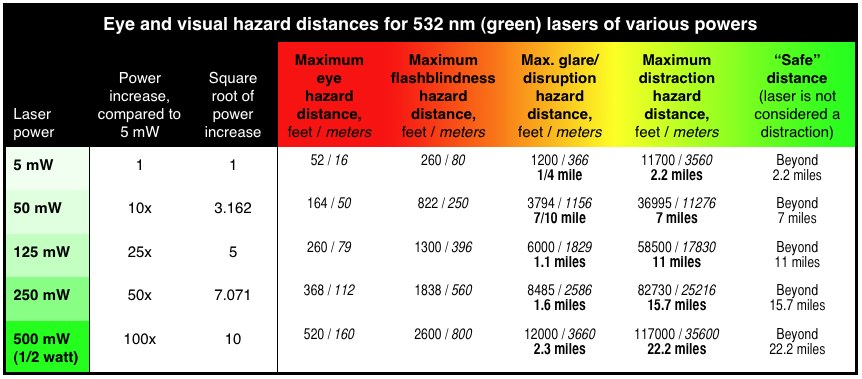
\includegraphics[scale = 0.5]{laserrange.jpg}
				\caption{Laser Range}
			\end{center}
		\end{table}
		
		\subsection{Buffer design}
		\begin{figure}[ht!]
			\begin{center}
				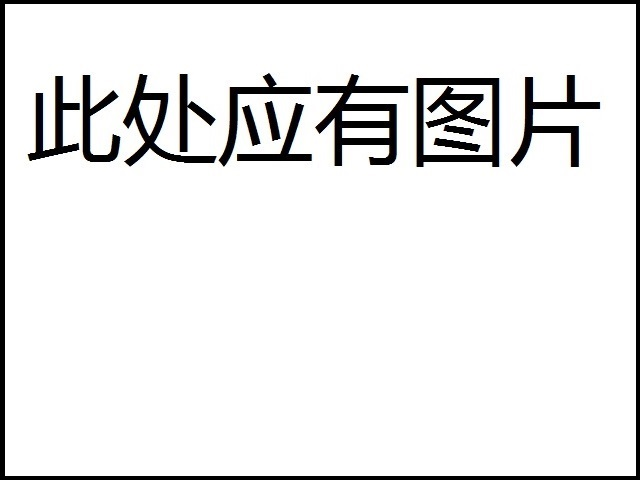
\includegraphics[scale = 0.6]{1D.jpg}
				\caption{Linear Sliding Track}
			\end{center}
		\end{figure}
		The actual design for the buffer is using the linear sliding track (Figure 3.3). There are two sides of the linear sliding track as the CAD shows in Figure 3.3. Side A connects to tractor and side B connect to camera and attachment tools. In addition, considering of the duty of tractor attachments is very heavy, the sliding track must be firm and the stepper motor must be powerful.
		
		In this built prototype, a lighter and smaller frame was used for convenience. And for the demonstration purpose, no other heavy agricultural attachments will be installed. The camera was mounted on the small sliding block of the frame. Then, a hood is attached on the camera with a curtain covered in front. Hood reduces noise by blocking out light from the angle that camera does not need to see. Curtain works like a projection screen, so that the laser pointer can leave a spot on it.  A stepper motor is installed on edge of the frame, and drive the block with camera with a belt. The power of stepper motor along with the control signal was given by a stepper motor driver board. 
		
		The center processor is a Raspberry Pi, it process the image captured by camera and then send the digital control signal to the stepper motor driver board. The wire connections shows in Figure 3.4.
		\begin{figure}[ht!]
			\begin{center}
				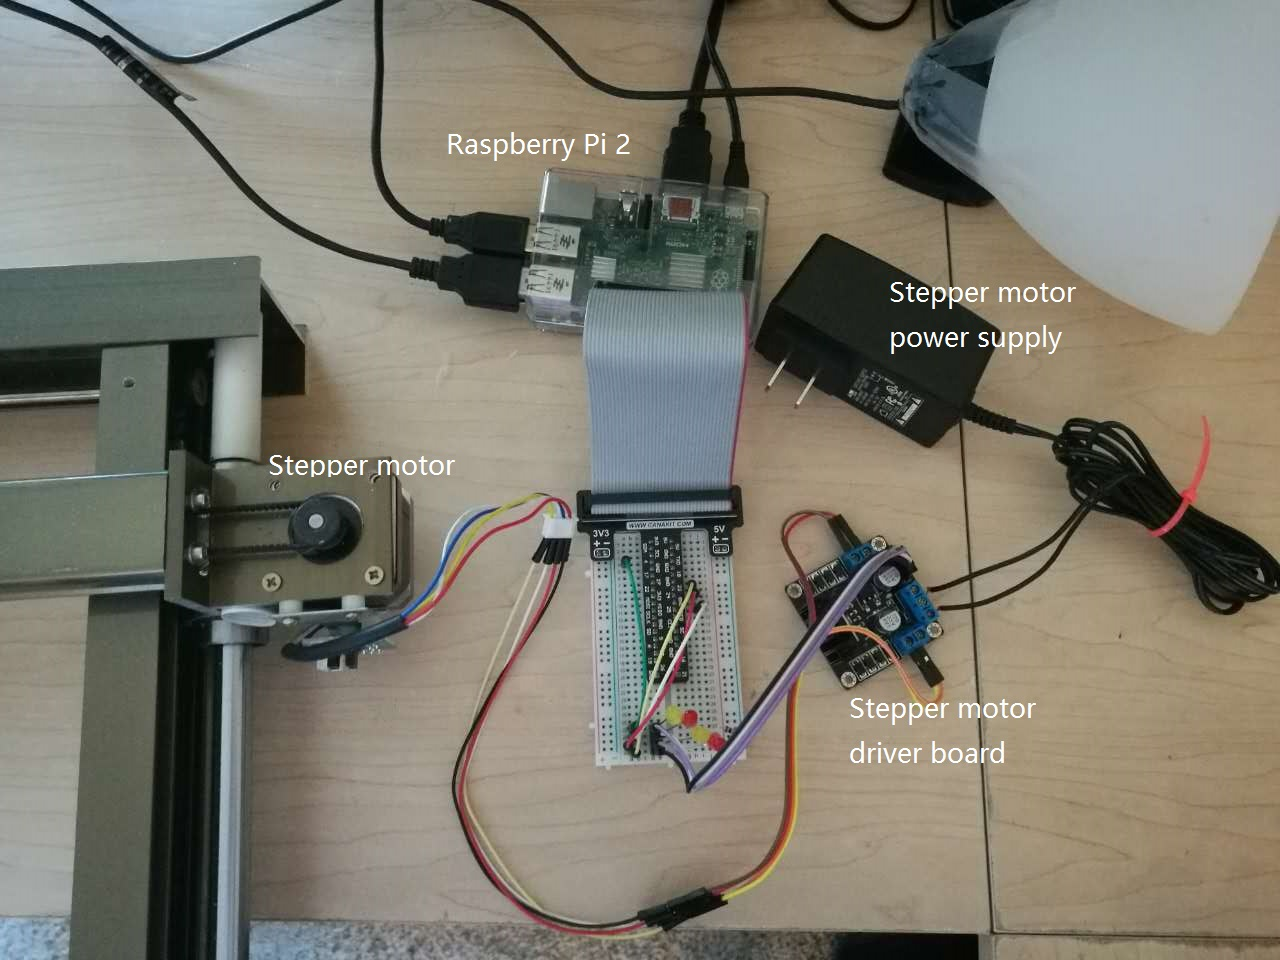
\includegraphics[scale = 0.4]{connection.jpg}
				\caption{Wire Connections}
			\end{center}
		\end{figure}
		The prototype works in the process as the flow chart (Figure 3.1) showed. At the beginning, point the laser pointer to the camera curtain. After the origin position initialized, move the frame. And the block with camera that assumed to also have other tractor attachment tools installed on will always stay stable. 
		
		
		\subsection{Image processing}
		\begin{figure}[ht!]
			\begin{center}
				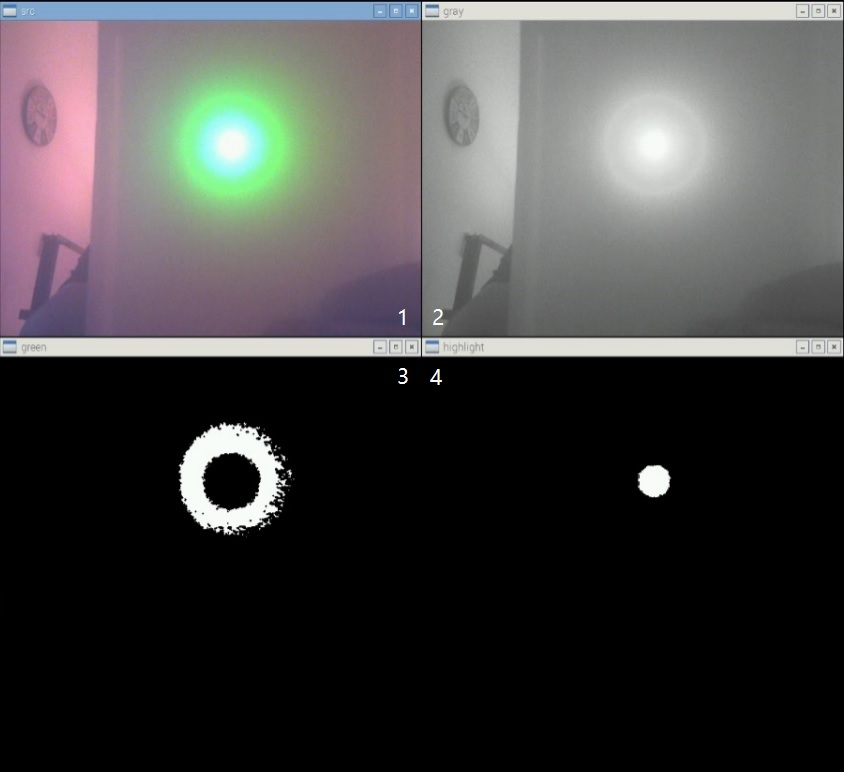
\includegraphics[scale = 0.7]{imaging.jpg}
				\caption{Image Processing}
			\end{center}
		\end{figure}
		Image processing algorithm is using to find the position reference from the data gathered by camera. The algorithm was written in C++ with OpenCV. There are several different ways were tested.
		
		\subsubsection{Color detection}
		
		Color detection was the first method that was implemented and tested. Color detection is straightforward and accurate. Generally, green should be a great color for detection. The reason is that green is the color with low showing frequency in our daily life, which is the same with why chroma key compositing technology always uses green as the background color. However, green could be everywhere in the crop field, so it is hard to detect the green laser with a green background. To solve this problem, a hood and curtain was attached to the camera to reduce the low intensity lights. Therefore, only the green laser able to leave a clear green spot on the sight of the camera. (Figure 3.5 - 1) Although the spot is clear green from human vision, it may not be recognized as green by camera. Under the RGB color space, the "green" spot is always mixed with bule, and sometime red. The color detection is very unreliable, because it could be affected by the surrounding light, thickness of the curtain, and other unknown factors.
		\subsubsection{color detection}
		
		According to a related research, HSV color space has achieved a more accuracy performance compared to the original RGB color space. \cite{kaur2013content} To improve the color detection, HSV color space was tested. RGB is well-known as red, green, and blue which are the primary colors of light. Every pixel on a picture contains these three values. Similar with RGB, the three values of HSV are hue, saturation, and value. Unlike the RGB color space that every the value has a same range from 0 to 255, the values of HSV color space have different ranges. Hue is the color type which is ranged from 0 to 360 degree. Saturation is ranged from 0 to 100 $\%$ as well as the value which is the brightness. RGB color space is based on Cartesian coordinate system, but HSV color space is based on cylindrical coordinate system. (Figure 3.6)
		\begin{figure}[ht!]
			\begin{center}
				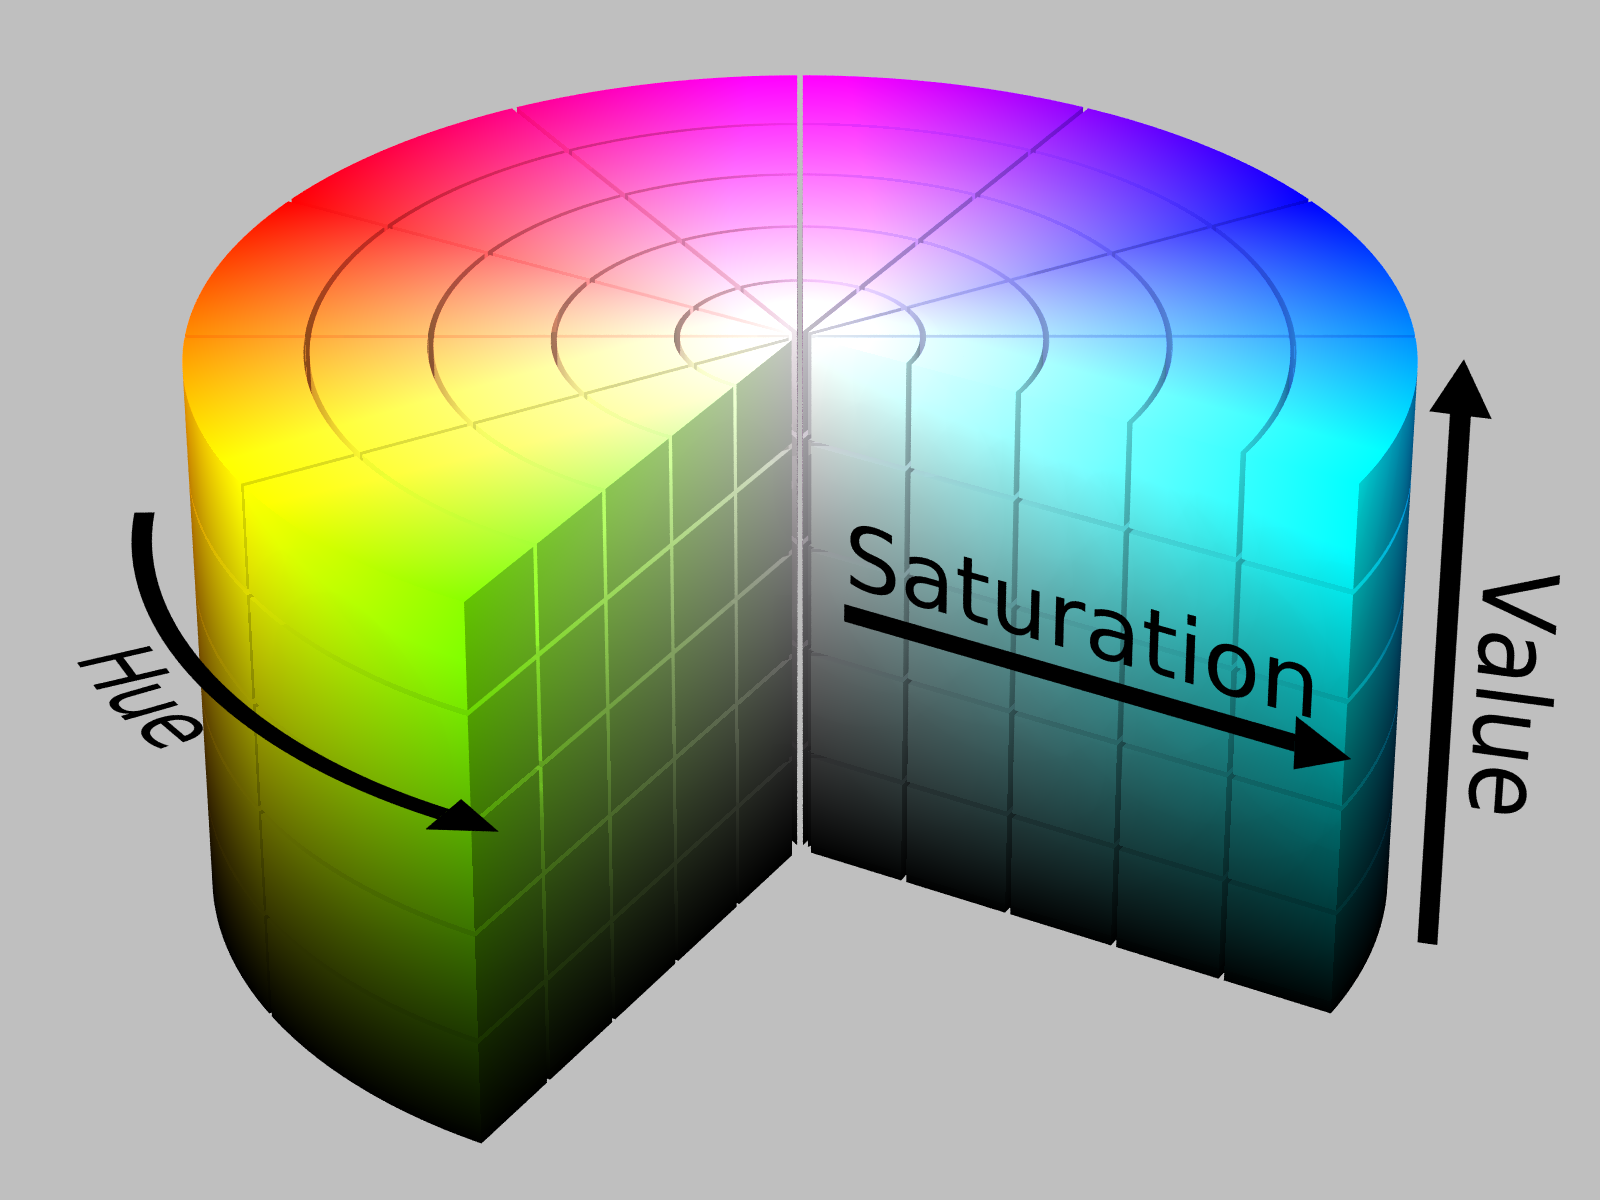
\includegraphics[scale = 0.2]{HSV.png}
				\caption{HSV Color Space}
			\end{center}
		\end{figure}
		
		The conversion formulas are
		\begin{equation}
			H = cos^{-1}(\frac{\frac{1}{2}[(R-G)+(R-B)]}{\sqrt{(R-G)^{2}+(R-B)(G-B)}})
		\end{equation}
		\begin{equation}
			S = 1-\frac{3}{R+G+B}(min(R,G,B))
		\end{equation}
		\begin{equation}
			V = \frac{1}{3}(R+G+B)
		\end{equation}
		After the original image has transfered from RGB to HSV, a ring shaped detection was showing on the screen. (Figure 3.5 - 3) The green color detection is stable this time under HSV color space. However, the ring shaped detection is unable to provide an accurate coordinate. Unfortunately, there is no way to detect green at the center, because the light intensity at the center is too high for the camera to detect any color.
		\subsubsection{High intensity detection}
		
		For the close distance detection, an additional algorithm was developed. This algorithm only  provides an accurate detection in a close range as a helper for the color detection. First, the original image was transfered from RGB to GRAY instead of HSV. (Figure 3.5 - 2) Then find the intensity bump by masking off all the pixels that is 20 units lower than the maximum intensity. As a result, the detection becomes a nice point. (Figure 3.5 - 4)
		
		\section{Improvement to the laser guidance}
		
		The buffer was designed as a linear buffer that can only provide the offset in the direction that is perpendicular to the tractor moving direction. However, tractor can not move left or right, it can only turn left or right. Therefore, after the sliding occurs, tractor have to turn to make the correction. In other words, there are some small angles between the planned direction and the actual direction while tractor is moving. In order to cancel these angles, this design needs some improvements.
		
		\subsection{Improvement to the buffer}
		\begin{figure}[ht!]
			\begin{center}
				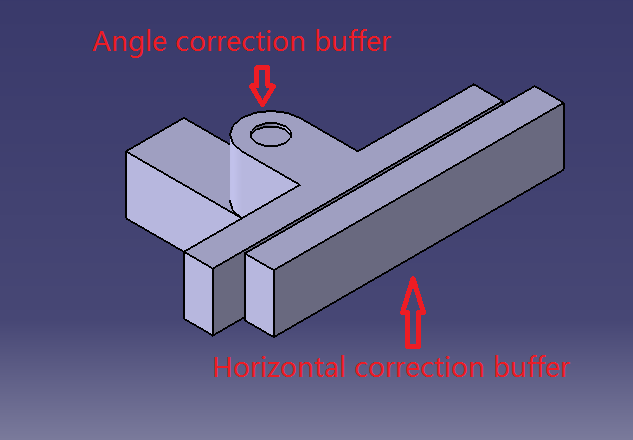
\includegraphics[scale = 0.8]{improvedbuffer.png}
				\caption{Improved Buffer}
			\end{center}
		\end{figure}
		Based on the previous design, one more stepper motor needs to be installed as the Figure 3.7 shown to provide the offset for the angle. The duty stepper motor is to provide a vertical spin to correct the angle error while that tractor is turning. 
		
		\subsection{Improvement to the curtain}
		\begin{figure}[ht!]
			\begin{center}
				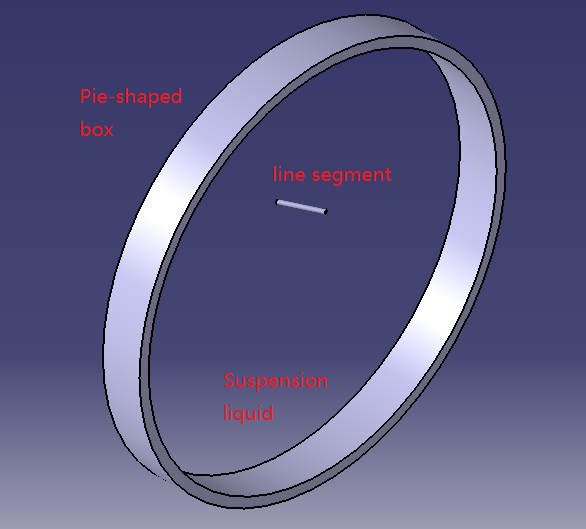
\includegraphics[scale = 0.8]{improvedcurtain.png}
				\caption{Improved Curtain}
			\end{center}
		\end{figure}
		Previously, it is introduced that the curtain works like a projection screen. The only trace that laser left is a spot. Under this situation, it is impossible to find the error angle just from one single spot. The new design for the curtain is a pie-shaped transparent plastic box which full filled with suspension liquid. Under the semi transparent environment, the trace of laser is no longer a spot, but a segment. (Figure 3.8) A segment provides more information than a single spot. It is able to find the angle with the direction and length of the segment.
		
		\subsection{Improvement to the algorithm}
		Base on the developed color detection algorithm, the image captured by camera shows a line segment. (Figure 3.9)
		\begin{figure}[ht!]
			\begin{center}
				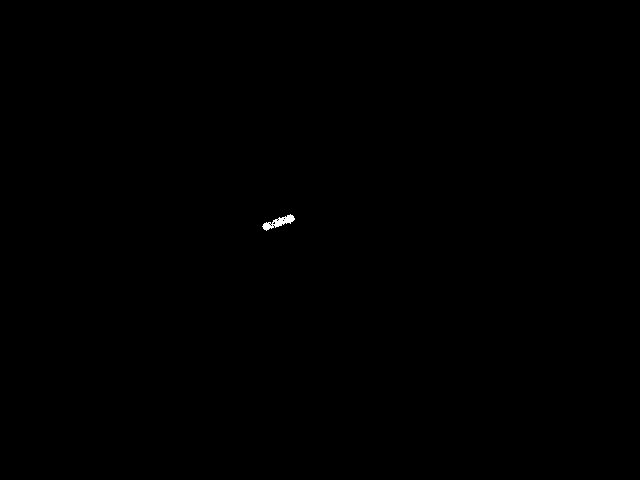
\includegraphics[scale = 0.6]{segment.png}
				\caption{Line Segment}
			\end{center}
		\end{figure}
		The improved algorithm finds the angle by the followed process. 
		\subsubsection{Coordinates for each end}
		
		The camera is monitoring the curtain slightly upward, so according to the perspective rule, the upper right end of the segment is the front. For example, the coordinate of upper right end is $(292,217)$, and the coordinate for the lower left end is $(265, 227)$ in Figure 3.9.
			
		\subsubsection{Projection length of segment}
			
		With the coordiantes of these two ending points, the projection length can be calculated as below. And the unit is pixel. 
		\begin{equation}
			L = \sqrt{(292-265)^2+(217-227)^2} = 29 \quad pixels
		\end{equation}
			
		\subsubsection{Thickness of the curtain}
			
		Since the position and the size of curtain are both fixed, thickness is a constant in this algorithm. This constant was found by taking a picture in the same distance and measuring the pixels on the picture. The thickness of the curtain is 56 $pixels$.
			
		\subsubsection{Error angle}
			
		Since the projection length of the segment and the thickness of the curtain are known from above calculations, the error angle can be calculated with trigonometric function as following.
		\begin{equation}
			Error Angle = tan^{-1}(\frac{29}{56}) = 27.38^o
		\end{equation}

		According to the perspective rule, the buffer was turned to the right for 14.84 degree. Therefore, this error angle can be corrected by turning the second stepper motor to the left for 14.84 degree. 
		
		\subsection{Vision guidance}
		Vision is one of the most important ways to collect information from surroundings for human, but it is still young for machines. Machines used to collect information from surroundings via tons of sensors. A lot of researchers study on imaging processing because it is believed that machine can do what ever human can do by just using camera as their only sensor. 
		
		It is only a tiny modification to the previous design to fit the vision guidance system instead of laser guidance system. Remove the curtain and the hood so that the camera is able to "see" open wide. And the laser pointer is no longer needed. Although it is an idea and nice guidance system that just using a camera, it is hard to achieve at this time. Crop field is different from either city roads or indoor factories. Crop field is an open area where is very hard to find a landmark as reference. This cannot be simply solved by place a distinctive object at the end of rows, such as a traffic cone. Referring an experiment has been made to test the feasibility for using traffic cone as an object reference. 
		\begin{figure}[ht!]
			\begin{center}
				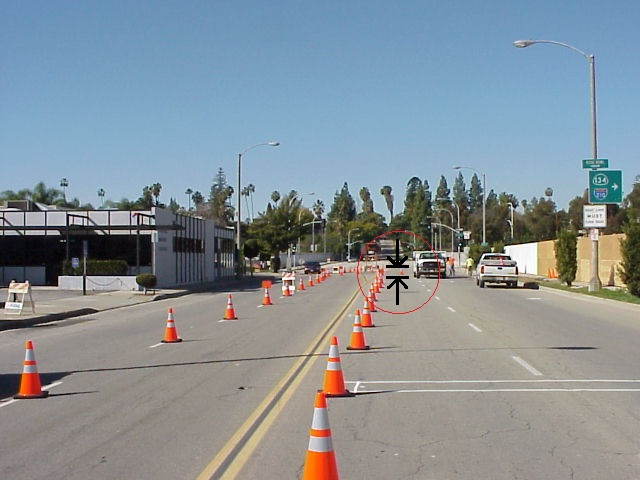
\includegraphics[scale = 0.8]{cone.jpg}
				\caption{Traffic Cones}
			\end{center}
		\end{figure}
		Figure 3.10 is a picture that in the resolution of $640\times480$ which is the same resolution with 480P camera. The distance to the marked farthest traffic cone in the picture is about 50 m, and the cone is 9 pixels high. The height of a traffic cone is about 75 cm and it becomes 9 pixels in the picture with 50 m distance. Typically a row in crop field in over 200 m, so it is very hard to detect the cone. From the result (Table 3.3) in a related research, at least $32\times32$ pixels are need to obtain an acceptable detect rate. \cite{torralba2009many}
		\begin{table}[ht!]
			\begin{center}
				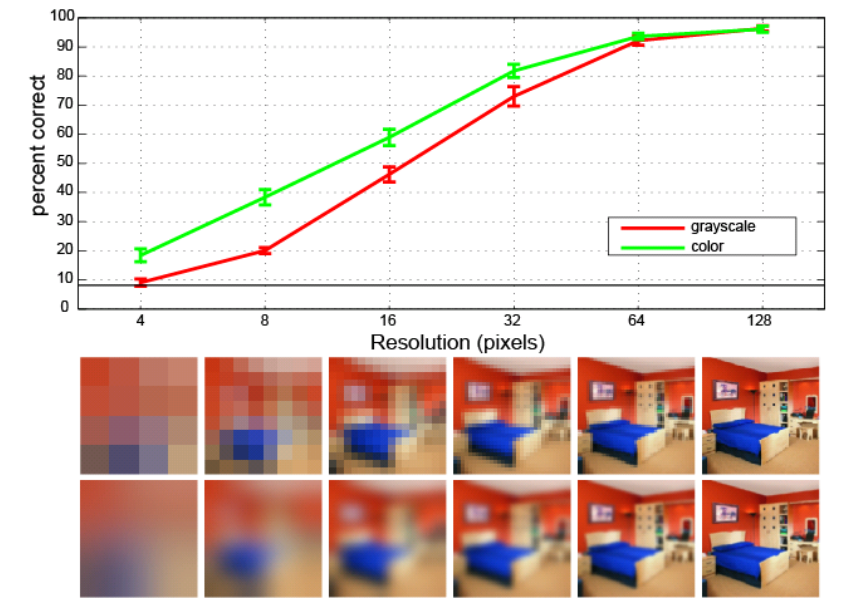
\includegraphics[scale = 0.6]{pixel.png}
				\caption{Resolution Vs. Recognition Probability}
			\end{center}
		\end{table}
		
		\subsubsection{High resolution camera}
			
		In order to obtain a $32\times32$ pixels traffic cone in 50 m distance, the original picture have to have a resolution that is 4 times in both length and width which is $2560\times1920$. The resolution of a 1080P camera is only $1920\times1080$ which is still not enough, so a 4K camera have to be used. However, a 4K camera is about \$ 300 which is over 8 times more expensive than the 480P camera. Even if the budget is permitted, a 4K camera will not be helpful if the distance is farther than 50 m.
		\subsubsection{Larger reference object}
			
		A large object is easy to be detected because of there are more pixels in the picture. It is obviously to tell from Figure 14, the object have to be as large as the trees, so the vision guidance might be able to work if there are trees at the end of crop field. However, this situation is not widespread.
			
		\subsubsection{Zoom lens}
			
		Although camera with zoom lens is able to take a clear picture from far distance, it is very expensive. And even with the zoom lens camera, taking clear picture from far distance requires stable condition, otherwise the picture will be blurry. A moving tractor obviously unable to provide that stable condition.
			
		\bigskip
		Therefore, there is no way to implement a vision guidance system for crop field under current situation. Laser guidance system is the best solution.
		
		\chapter{Results}
		
		\section{Introduction}
		This paper introduced a new guidance system design for agricultural machinery. This design contains a buffer and a laser pointer. The buffer is a device that needs to be install on tractor attachment. And the laser pointer needs to be placed at the end on crop field rows facing to the back of the tractor. The usage of this guidance system is placing the laser pointer at the right position and face the right direction firstly. Then project the laser to the curtain of the buffer. After the buffer has initialized, the tractor is ready for the farm operation. It is not only suitable for the existing GPS guided agricultural machinery, but also work on the ones that without any guidance system on board to enhance the accuracy from $\pm$ 10 cm to $\pm$ 2 cm. The only difference is addition LEDs needs to be installed on the dash board of the tractor. If the driver can drive at a low speed and handle the steering wheel carefully based on the signal on the dash board which given by the laser guidance system, it is expected to have the same $\pm$ 2 cm accuracy. 
		
		%使用这个设备能达到那些效果。为农业育种提供方便,为未来的无人农业提供先决条件。
		
		\section{Technical highlights}
		
		\subsection{Local laser reference}
		The guidance system introduced by this paper is using laser as a local reference. A local reference is able to provide a more reliable guidance because there are less noise factors. For instance, GPS is based on the distance measurement between several satellites and a receiver, the high atmosphere has a significant affect to its accuracy. 
		
		\subsection{Buffer}
		The method that this guidance correct error is to install a buffer to the tractor attachment. The method that current technology make correction is to turn the steeling wheel of the tractor. This method is inefficient, because no matter how fast the correction can be made, the deviation of trajectory exists. However, deviations will never take place with the buffer installed on the tractor attachment. The buffer always stay at a relatively steady position with the laser reference. It allows the tractor deviates for a little bit while keeping the trajectory on the right track before the tractor made its correction.
		
		\subsection{Image processing}
		The algorithm contains two parts. High intensity detection is using when the tractor is close to the laser pointer. The laser pointer is designed to have range that is over 200 $m$, so it is very bright at a close distance. High intensity detection provides a more stable detection because it is too bright to detect color. Once the color detection show a stable result, high intensity detection will be disabled. 
		
		%利用摄像头来引导是趋势,摄像头成本低,易于改进,人就是靠视觉获取信息,同样机器也可以
		
		\section{Feasibility}
		The laser guidance system introduced in this paper is an add-on device to the current tractor attachments. Users does not need to buy either new tractors nor attachments, just two parts of this device. Therefore, the cost is very low. However, the set up procedure is a little bit complex. Therefore, it may not be the best choice to spread out to every farm because of the 76.2 $cm$ row spacing still the mostly in use. The best place to apply this design is the experimental crop field which goal is find the high performance breed. The seeding position is very strict, so that different breeds are comparable because of the identical growth environment of every plant. 
		
		In the future, the row spacings will be as narrow as possible so that more crops can be planted. High accuracy agriculture machinery is necessary for every corner of the world. The advantage of laser guidance system is that every machinery on duty is able to upgrade. It is not necessary to buy brand new tractor which has GPS guidance system on board and then upgrade based on GPS. Therefore, laser guidance system is a great choice for most of the developing country where GPS tractor is not popular. It is a very economic deal for them to achieve the precision agriculture.
		
		
		\section{Constraints}
		The guidance system that introduced is base on image processing algorithm. Therefore, any condition that affect the camera will affect this system. The most common problem is the dust cause by the running tractor. Heavy dust may block the laser light and cause the guidance loose reference. As for the laser light, 5 $mW$ green laser pointer is in use for now and higher power laser pointer may be used in the future to provide a farther distance reference. Therefore, safety is a big problem because the high power laser is able to damage retina in a close distance. Furthermore, it is very important to set up the laser pointer in the correct direction. A small error of angle will cause a big difference because of the long column distance. According to these two reasons, it is necessary to have a trained operator. At last, since the limited resources and time, this guidance system is only designed for flat land. It will not work on sloping fields.
		
		
		\section{Application to other areas}
		Essentially, the design of the paper is guidance system. Therefore, the laser guidance system can not only apply in agriculture machinery, but also apply any other outdoor vehicles that need a precision guidance. In the aspect of agriculture, the buffer only stabilize horizontal direction. In fact, the buffer can also be stabilize vertical direction. This feature can be applied to the cart that move fragile materials on a bumpy ground. For example, the outdoor AGVs with the laser guidance system are able to move fragile materials, such as glasses, around the construction area just like indoor ones working in a factory. 
		
		\chapter{Conclusion}
		
		\section{Importance of outdoor-AGV}
		Outdoor AGV is an essential and practical in the future of modern agriculture. Most of the current AGV in application is for indoor use, which is not applicable for outdoor environment. In the outdoor condition, various problems would occur that are mentioned such as rough ground, unpredictable weather and high expense of equipment, which is very different from indoor condition. Furthermore, since most of guidance systems of indoor AGV requires pre-set wires, magnets, or paints, it is very expensive and inconvenience to use them outdoor. Therefore, it is urgent to developed a feasible AGV for outdoor using. In this paper, it is mainly focused on the straight rowing on the field. The significance of planting crop on the straight line is to control the same condition for all areas in the experiment as well as to lay the foundation on further agriculture purpose such that straight rowing would reduce the work of irrigation by control the position of irrigation and create convenience for agriculture robots. Hence, the development on laser-Guided Automatic Vehicle can solve both problems mentioned and inspire more ideas on outdoor AGV researches.
		%本文重点讨论了关于户外AGV在农业方面的应用,现在工厂有流水线,但是室外的农业却没有这么高效率。目前来说,传统的GPS农机或许在播种上能满足现在的需求。但是要满足育种试验田的播种需求,还是需要户外AGV。放眼未来,要实现想工厂流水线一样高效的无人农业,精准的播种是第一步也是非常重要的一步。
		
		\section{Overview of significants}
		The laser guidance system introduced in the paper is accurate and economic method to guide the outdoor vehicles. There are two devices of this guidance system, one of them is the laser pointer, and the other one is the buffer. Laser pointer emits straight laser light which provides the reference for the guidance system. Its position is fixed on the ground and pointing to the direction that vehicle needs to move. The buffer is installed on the vehicle to provide the guidance. There is a camera on the buffer which is used to receive the laser light reference, and then the on board microprocessor analysis the information by running the designed algorithm. Finally, microprocessor sends action commands out. In this paper, these commands are sending to buffer to stabilize the tractor attachment, as well as to the driver if there is no GPS guidance system on board. For other aspects, these commands not only guide the movement of the vehicle, but also can stabilize the cargo that was carried by the AGV. It is very useful if the AGV is transporting fragile materials on a dumpy ground.
		
		
		\section{Limitations}
		Laser light travels in a straight line, so the this guidance system which use the laser light as a reference is only good at moving in straight line. In order to make turns, it have to have an additional guidance system on board, such as GPS, to cooperate. Moreover, one laser pointer have to be set for each segment of straight route. On the other hand, the laser guidance system will also be lost if the route is not monotonically up or down. Imagine the situation that vehicle goes uphill firstly and then go downhill, the laser pointer can only guide the former movement. Therefore, there is a limitation in the geography of the working area.
		
		The camera on the vehicle observe the laser light as a reference, but it might hard to "see" the laser light under some situations. The observation will be affected by the surrounding lights. When use this guidance system outdoor, the main factor that affect the laser light detection is the strong sun light. If the light intensity of surroundings is too high, laser light could be polluted so that green color is unable to be detected. Therefore, it might be required to operate during early morning or in the late afternoon when the sun light is weak. 
		
		\section{Further improvement}
		Based on the limitations, the laser guidance system can be improved in two ways in the future. First, adapting to diverse geography working area. On the one hand, since some of crop fields are circle shaped for the convenience of the giant irrigation sprinklers, it is better to plant the crops in the same shape. On the other hand, not all of the crop fields are flat. In fact, some of farm land is even in the mountain area. It is very necessary to make the guidance system able to work on every kind of farm. Second, reduce the affect from the strong sun light. Farming operations are generally taking place during the day. Furthermore, most of the crops require a very limited time window to be planted. In order to apply the laser guidance system widely, it will be more convenience if the guidance system is able to work properly any time. 
		
		\bibliographystyle{ieeetr}
		\bibliography{mybibfile}
		\addcontentsline{toc}{chapter}{Bibliography}
		
		\backmatter
		\begin{appendices}
			\appendixpage
			\noappendicestocpagenum
			\addappheadtotoc
			
			\chapter{Appendix A}
			Some text
		\end{appendices}

\end{document}